\documentclass[aspectratio=169]{beamer}

\usefonttheme{serif}

\usepackage{physics}
\usepackage[export]{adjustbox}
\usepackage[absolute,overlay]{textpos}
\usepackage{graphicx}

\title{Kiral perturbasjonsteori}

\author{Martin Johnsrud}

\begin{document}
    % \frame{\titlepage}

    \begin{frame}
        \frametitle{Kan pioner danne stjerner?}
        \begin{itemize}
            \vspace{-3cm}
            \item Nylig: forslag om at pioner kan danne stjerner
            \item Kvantekromodynamikk, QCD, er teorien om hvordan kvarker vekselvirker via kjernekraften, også kalt sterk vekselvirkning
            \item Bindes til baryoner (f.eks. protoner, nøytroner) og mesoner (f.eks pioner)
            \item Må beskrives med effektive teori: bytter ut kvarker/gluoner med baryoner/mesoer
        \end{itemize}

        \begin{textblock}{6}(8.5, 7)
            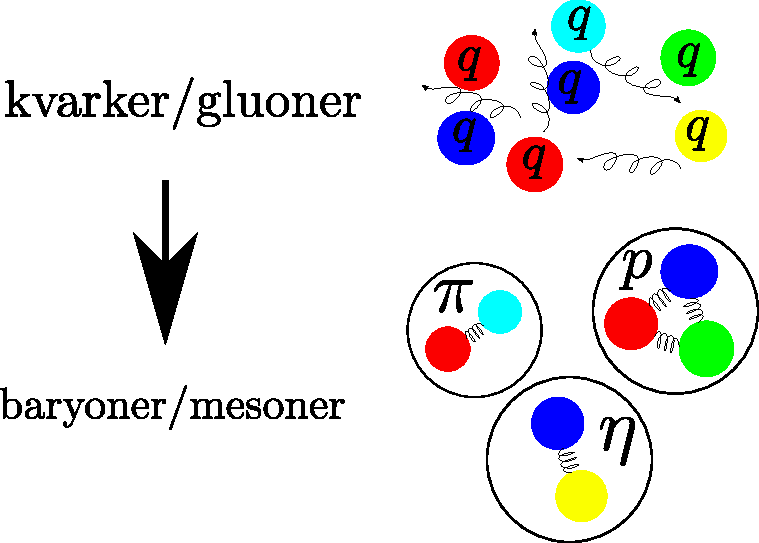
\includegraphics[width=\textwidth]{figurer/quarks-to-mesons.pdf}
        \end{textblock}

        \scriptsize{
        \begin{textblock}{10}(1,8.5)
            $
            \mathcal L = 
            \sum_f \bar q_f (\gamma^\mu [\partial_\mu - i q \lambda^a A^a_\mu ] + m_f)q_f
            + G^a_{\mu \nu} G_a^{\mu \nu}
            $
        \end{textblock}

        \begin{textblock}{8}(1, 12)
            $
            \mathcal L_\text{eff}
            =
            \frac{1}{4} f^2 \Tr{\nabla_\mu \Sigma (\nabla^\mu \Sigma)^\dagger}
            + \frac{1}{4} f^2 \Tr{\chi^\dagger \Sigma + \Sigma^\dagger \chi} 
            % + \frac{1}{3} l_1 \Tr{\nabla_\mu \Sigma (\nabla^\mu \Sigma)^\dagger}^2+
            ...
            $
        \end{textblock}
        \begin{textblock}{15}(1, 13)
            $
            \Sigma(x) = \exp{ i \frac{1}{2f} \pi_a(x) \tau_a}
            $
        \end{textblock}
        
    }
    \end{frame}

    \begin{frame}

        \frametitle{Termodynamikk}
        \begin{columns}

            \begin{column}{0.6\textwidth}
                \begin{itemize}
                    \vspace{-1cm}
                    \itemsep 0.8cm
                    \item Fri energi i storkanonisk ensemble,
                    $
                    F = - T
                    \ln[\int D \pi \, 
                    \exp(i \int \dd^4x \, \mathcal L + i \mu_I Q_I )]
                    $
                    \item $Q_I$: isospin, $\mu_I$: kjemisk potensiale
                    \item Et system i likevekt vil minimere fri energi
                    \item Når kjemisk potensiale er lik massen til pionene skjer en faseovergang 
                \end{itemize}
            \end{column}

            \begin{column}{0.5\textwidth}
                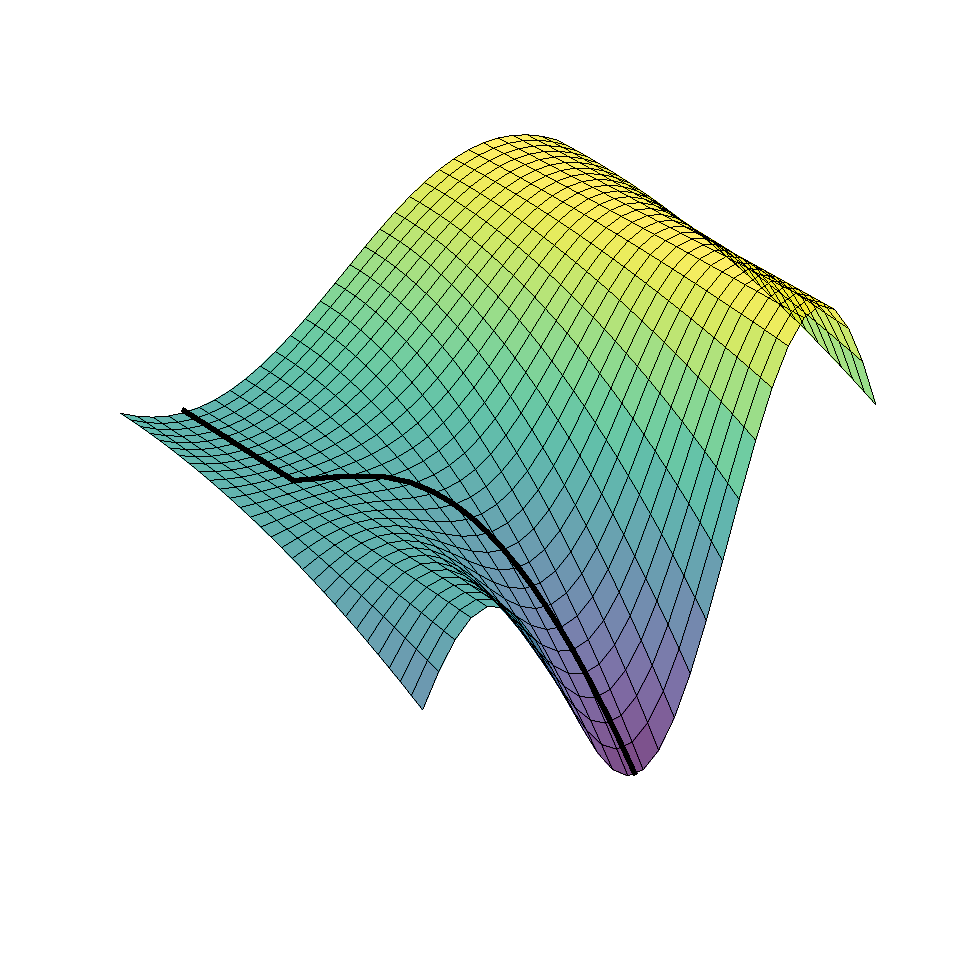
\includegraphics[width=1\textwidth]{figurer/numerics/free_energy_surface_wo_axis.pdf}
            \end{column}

        \end{columns}

    \end{frame}

    \begin{frame}
        \frametitle{Pionkondensat}
        \begin{columns}
            \begin{column}{0.6\textwidth}
                \begin{itemize}
                    \vspace{-0.5cm}
                    \itemsep 0.8cm
                    \item Vil få en grunntilstand hvor $\langle \pi \rangle \neq 0$, selv ved $T = 0$
                    \item Danner et Bose-Einstein kondensat
                    \item Hypotese: kan danne stjerner
                    \item Trenger tilstandsligning, relaterer trykk og energitetthet $f(u, P) = 0$
                    \item (Ja, vi antar stjerner har $T=0$, men det går greit. Stol på meg)
                \end{itemize}
            \end{column}
            \begin{column}[]{0.5\textwidth}
                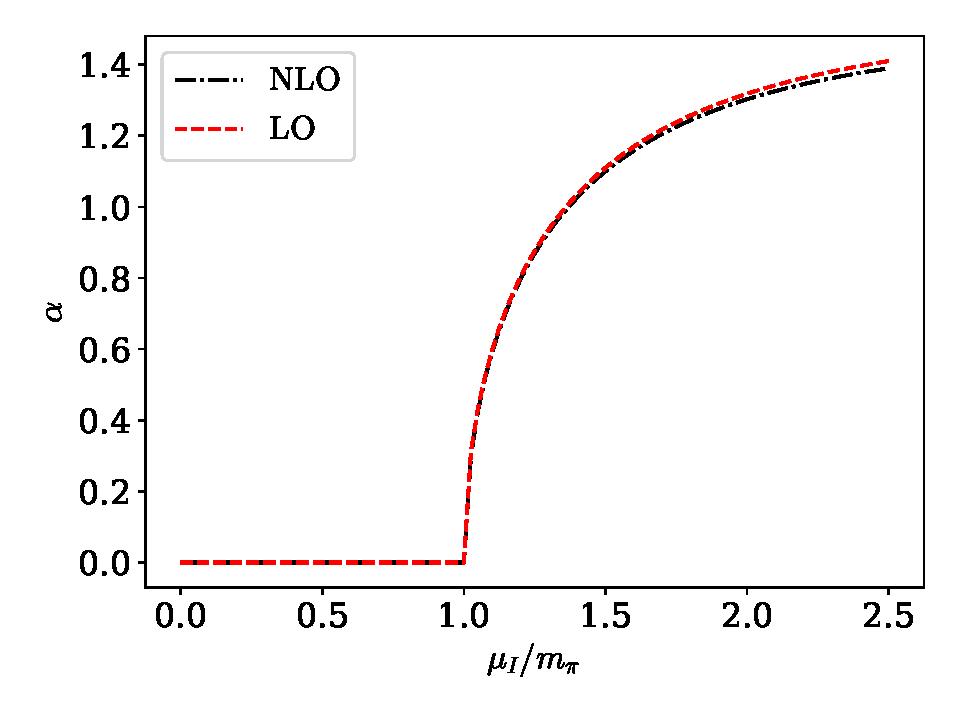
\includegraphics[width=0.88\textwidth]{figurer/numerics/alpha.pdf}
                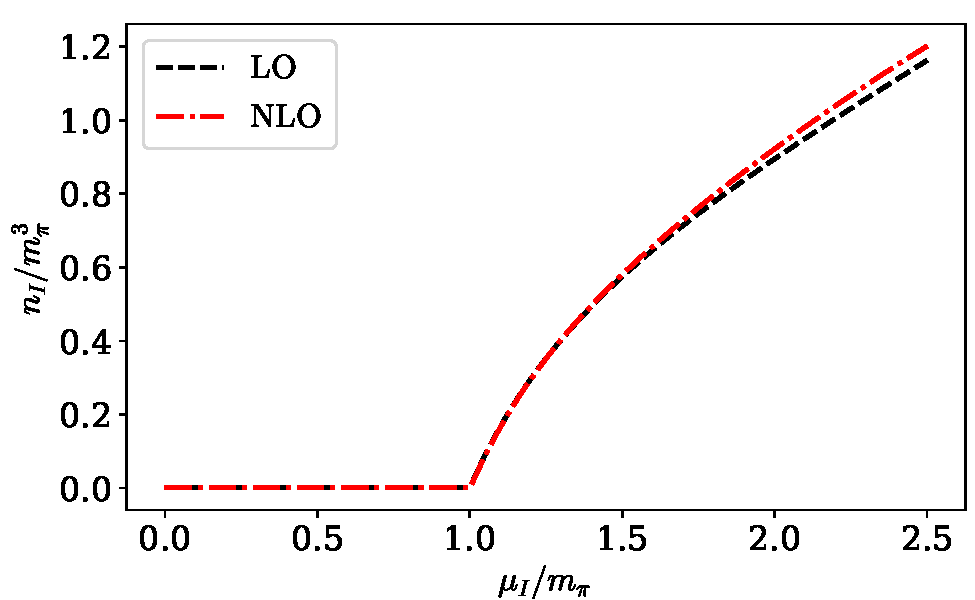
\includegraphics[width=0.88\textwidth]{figurer/numerics/isospin_density.pdf}
            \end{column}
        \end{columns}
        \end{frame}

    \begin{frame}
        \frametitle{Tilstandsligning}
        \centering
        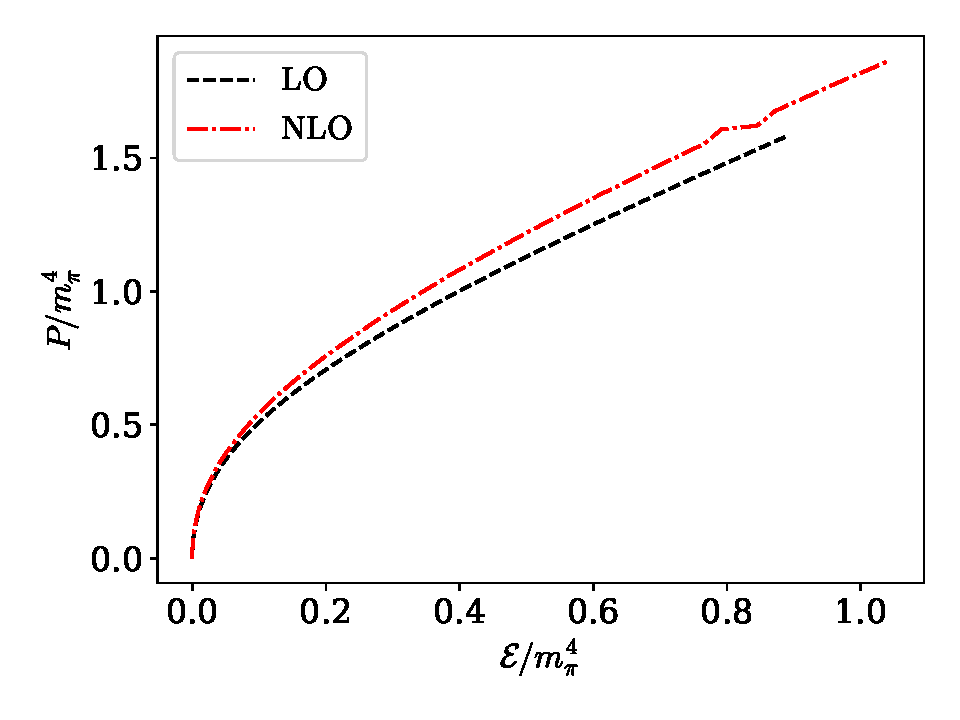
\includegraphics[width=0.8\textwidth]{figurer/numerics/energy_density.pdf}
    \end{frame}

\end{document}
